\documentclass[tikz,border=5pt]{standalone}
\usepackage{tikz}
\usetikzlibrary{positioning,calc}
\usetikzlibrary{arrows.meta}

\begin{document}
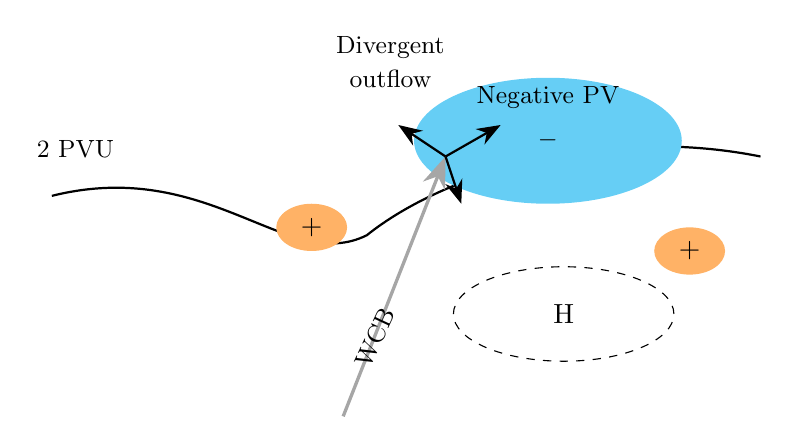
\begin{tikzpicture}[scale=1,>=Stealth]

% Tropopause (2 PVU)
\draw[thick]
(-4,0.3) .. controls (-2,0.8) and (-1,-0.7) ..
(0,-0.2) .. controls (1,0.6) and (3,1.2) ..
(5,0.8);

\node at (-3.7,0.9) {\small 2 PVU};

% Blocking high
\draw[dashed] (2.5,-1.2) ellipse (1.4 and 0.6);
\node at (2.5,-1.2) {H};

% Negative PV anomaly
\fill[cyan!60] (2.3,1.0) ellipse (1.7 and 0.8);
\node at (2.3,1.0) {\small $-$};
\node at (2.3,1.55) {\small Negative PV};

% Positive PV anomalies
\fill[orange!60] (-0.7,-0.1) ellipse (0.45 and 0.3);
\node at (-0.7,-0.1) {$+$};

\fill[orange!60] (4.1,-0.4) ellipse (0.45 and 0.3);
\node at (4.1,-0.4) {$+$};

% Warm conveyor belt
\draw[very thick,gray!70,-{Stealth[length=4mm]}]
(-0.3,-2.5) -- (1.0,0.8);

\node[rotate=65] at (0.1,-1.5) {\small WCB};

% Divergent outflow
\draw[thick,-{Stealth[length=3mm]}]
(1.0,0.8) -- (0.4,1.2);

\draw[thick,-{Stealth[length=3mm]}]
(1.0,0.8) -- (1.7,1.2);

\draw[thick,-{Stealth[length=3mm]}]
(1.0,0.8) -- (1.2,0.2);

\node[align=center] at (0.3,2.0)
{\small Divergent\\\small outflow};

\end{tikzpicture}
\end{document}